
\documentclass[12pt, a4paper]{article}
\usepackage{ragged2e}
\usepackage[margin=1in]{geometry}
\usepackage[utf8]{inputenc}
\usepackage[capposition=top]{floatrow}
%\usepackage[tablesfirst,nolists]{endfloat}
\usepackage{times}
\usepackage[flushleft]{threeparttable}
\usepackage{hyperref}
\usepackage{authblk}
\usepackage{setspace}
%\usepackage{apacite}
\usepackage{url}
\usepackage{caption}
\usepackage{graphicx}
\usepackage{titlesec}
\usepackage{color}
\usepackage{endnotes}
\usepackage{caption}
\usepackage{textcase}
\usepackage{booktabs}
\usepackage{titling}
\usepackage{rotating}
\usepackage{authblk}
\usepackage[toc,page]{appendix}

\captionsetup{
  labelsep=newline,
  justification=raggedright,
  singlelinecheck=false
}

\pagestyle{myheadings}
\title{}
\author{}
\date{}
\doublespacing
%\renewcommand{\efloatheading}[1]{}


\titleformat{name=\section,numberless}[hang]
   {\bfseries}{}{6pt}{\Large}


\let\footnote=\endnote


\bibliographystyle{vancouver}
\begin{document}

\title{The link between national football tournaments and alcohol-related domestic abuse - evidence from England}

\author{Anna Trendl$^{a,*}$ \\ \href{mailto:a.trendl@warwick.ac.uk}{a.trendl@warwick.ac.uk}\\
 \and Neil Stewart$^b$ \\ 
 \href{mailto:neil.stewart@wbs.ac.uk}{Neil.Stewart@wbs.ac.uk}
 \\ 
 \and Timothy L. Mullett$^b$ \\
 \href{mailto:Tim.Mullett@wbs.ac.uk}{Tim.Mullett@wbs.ac.uk}
 \\}
 
\date{
    $^a$Department of Psychology, University of Warwick, University Road, Coventry, CV4 7AL, United Kingdom\\
    $^b$Warwick Business School, University of Warwick, Scarman Road, Coventry, CV4 7AL, UK\\
    $^*$Corresponding author\\[2ex]%
    \today
}



\begin{titlepage}
%The cover page should include the title, running head, all authors’ names and affiliations (including departments), and full contact information for the corresponding author.

\maketitle
\thispagestyle{empty}
\centering
    This research did not receive any specific grant from funding agencies in the public, commercial, or not-for-profit sectors.
\clearpage
\thispagestyle{empty}
\RaggedRight
\begin{center}
\LARGE{The link between national football tournaments and alcohol-related domestic abuse - evidence from England}
\end{center}
\begin{abstract}
\noindent

%The abstract should be on a separate page and be no longer than 150 words. Five to seven relevant keywords should be listed directly under the abstract on the same page.


\textbf{Background.} Domestic abuse is increasingly recognised as a serious public health concern worldwide. In the context of England, previous research has suggested that the number of domestic abuse cases reported to the police increase on days when the national football (soccer) team participates in international football tournaments such as the World Cup. Alcohol is hypothesized to be an important factor in this relationship, but its exact role has not been explored yet. We sought to fill this gap by investigating the extent to which alcohol contributes to the link between football and domestic abuse.


\textbf{Methods.} Using a detailed crime dataset recorded between 2010 and 2018 by the third largest police force in England, we conducted a series of negative binomial regressions to investigate the relationship between England's participation in national football tournaments and the daily number of recorded alcohol-related domestic abuse incidents.


\textbf{Findings.} Our results show that the number of reported alcohol-related domestic abuse cases increases by 61\%, 95\% CI [32\% -- 96\%] following an England victory, while there is no comparable increase in the number of non-alcohol related domestic abuse cases. This is a large effect, translating into a 0.43 increase in the daily rate of alcohol-related cases per 100,000 individuals, against a base rate 0.71 cases per 100,000. This effect is specific to male-to-female cases, survives various robustness checks, and its time course is strongly consistent with a causal link between England's victory and an increase in alcohol-related domestic abuse.


\textbf{Interpretation.} Alcohol plays an instrumental role in the link between football and domestic abuse. Temporally targeted campaigns could be effective in raising awareness of the adverse effect of football-induced alcohol consumption on the prevalence of domestic abuse.


\textbf{Funding.} None.
\end{abstract}

\newpage
\thispagestyle{empty}
\textit{\textbf{Research in context}}


\textbf{Evidence before this study} While the link between football, masculinity and domestic abuse have been the focus of considerable scientific research, the exact role of alcohol in this relationship has not been explored yet. We searched the Wiley Online Library, Web of Science, and Google Scholar databases using the search terms \textit{football} and \textit{domestic abuse}, covering the period between 1995 and 2019. We have identified two relevant quantitative studies investigating the link between international football tournaments and domestic abuse, both of which used data from England. One study, using data from the 2010 World Cup, has found that the number of recorded domestic abuse cases increased significantly on England win and loss days, compared to various baseline days. Another study used data from the period of the 2002, 2006, and 2010 World Cups, and found that the number of recorded intimate partner violence cases increase 38\% when England loses, and 26\% when England wins or draws, compared to non-match days. To the best of our knowledge, our study is the first to explore the specific role of alcohol in the nexus between football and domestic abuse.


\textbf{Added value of this study}
Using 8 years' worth of detailed crime data from the third largest police force in England, we conducted the most comprehensive investigation of the link between football, alcohol, and domestic abuse up to date, and show that England's participation in international football tournaments results in an increase in the number of alcohol-related domestic abuse cases recorded by the police. We show that the time course of this increase is highly consistent with a causal link between football and alcohol-related domestic abuse. Furthermore, we reconcile our findings with previous, seemingly conflicting results, and demonstrate that it is an England victory, and not and England loss that results in an increase in the number of alcohol-related domestic abuse cases. Our results contribute to the scientific understanding of the factors precipitating domestic abuse.

\textbf{Implications of all the available evidence}
Alcohol consumption is key to the link between football and domestic abuse in England. Public information campaigns raising awareness of this problem could be the first step to reduce the public health risk associated with increased alcohol consumption following an England victory.

\end{titlepage}



\newpage
\RaggedRight
\section*{Introduction}

Domestic is increasingly recognised as a major public policy concern in many countries, including the UK \cite{ep}. While anyone can become a victim of domestic abuse, women are disproportionately affected, with more than 25\% of women, and 15\% of men in England and Wales reported to have experienced some form of domestic abuse since the age of 16 \cite{ONS}.

The link between sporting events and domestic abuse has been the focus of a number of smaller studies \cite{Williams2014}, but large-scale quantitative investigations of this relationship are relatively scarce. In England, previous studies have focused on the link between football (soccer) and domestic abuse. Football's history is inextricably linked to England, and it is by far the most popular sport in the country \cite{Parry2014}, with the 2018 World Cup attracting a record number of 44.5 million viewers \cite{BBC}. These studies have found significant increases in the number of domestic abuse cases recorded by the police on England win, and particularly on England loss days \cite{Brimicombe2012, Kirby2014}. While domestic abuse is predominantly understood as a pattern of ongoing behaviour involving a series of occurrences, rather than a one-off incident triggered by football \cite{Brooks-Hay2018}, these studies, and other qualitative investigations \cite{Swallow} nevertheless suggest that national football tournaments can create an environment for abusers that is conducive to domestic abuse.


%Two studies have investigated the effect of England's participation in the World Cup on the number of reported domestic abuse incidents. Using data on the number of reported domestic abuse cases in the month of the 2010 World Cup tournament, one study has found that the number of reported domestic abuse cases increased significantly when England lost or won (about 33-35\%), but did not change on days when they drew \cite{Brimicombe2012}. Another study has used daily count data from the 2002, 2006 and 2010 World Cups, and found a 38\% increase in the number of reported domestic violence cases when the England team lost, and a 26\% increase when they won or drew \cite{Kirby2014}. These figures were also quoted in a poster campaign launched before the 2018 World Cup, aiming to raise awareness of the link between football and domestic abuse \cite{NCDV}. While domestic abuse is predominantly understood as a pattern of ongoing behaviour involving a series of occurrences, rather than a one-off incident triggered by football \cite{Brooks-Hay2018}, these studies, and other qualitative investigations \cite{Swallow} nevertheless suggest that national football tournaments can create an environment for abusers that is conducive to domestic abuse.


Why would national football tournaments, such as the World Cup or the European Championship precipitate domestic abuse? England's participation in these tournaments are times of heightened patriotic emotions and a strengthened sense of ``Englishness'', fuelled by media narratives that often use war references, and a ``us vs. them'' rhetoric to generate and represent an English national identity \cite{Vincent2014}. Previous qualitative research has suggested that televised contact sports can serve as vehicle for the male sports fan to redefine, and express his masculinity in a way that allows dominance, control, and can ultimately manifest in the perpetration of domestic abuse \cite{Sabo,Swallow}, given susceptibility to such behaviours. We speculate that this observation is especially pertinent in the context of England's participation in national football tournaments, owing to the popularity of the sport in the country, the associated media attention, and the resulting heightened sense of national consciousness.

Qualitative investigations suggest that alcohol has a strong association with domestic abuse \cite{Peralta2010}: those with alcohol-problems are more likely to be perpetrators and, when alcohol is involved, there is evidence that the violence might result in more serious injuries. However, it is generally understood that the role of alcohol should be considered in the context of a range of social, biological and pyschological factors, and that alcohol is not the direct cause of domestic abuse \cite{Javaid2015,Peralta2010}. It has been suggested that for some men, drinking and violence plays an instrumental role in the construction and expression of masculinity, especially when the problem of masculine deficiency is present (e.g., by unemployment; \cite{Peralta2010}), some perpetrators use alcohol as a ``shield'' that protects them from being seen as a violent abuser and deflect responsibility \cite{Javaid2015}. 


Despite the well-documented connection between alcohol and domestic abuse, the role alcohol plays in the link between football and domestic abuse has not yet been explored. Given the strong association between drinking culture and football in England \cite{Dixon2014}, a relationship continuously reinforced by the marketing practices of the alcohol industry \cite{Gornall2014}, we conjecture that alcohol plays an important role in the link between national football tournaments and the well-documented increase in domestic abuse. Exploring the role alcohol plays in this relationship will deepen our understanding of the pathway through which football increases propensity for violence.

To investigate this question, we test if the daily number of reported alcohol and non-alcohol related domestic abuse cases recorded by the West Midlands Police (WMP) in England between 2010 and 2018 increase on days when the England national team plays in a national football tournament, and whether the effect depends on the result of the match. Since most England match days are allocated randomly (at least in the initial, group stage), national football tournaments are suitable for testing the effect of England matches on domestic abuse.  Our rich dataset further allows us to conduct a thorough investigation of the characteristics and temporal pattern of the domestic abuse perpetrated on England match days, and extend our findings in different directions. We also test the robustness of the effect using various model specifications, time periods, and geographical areas. 



\section*{Methods}


\subsection*{West Midlands Crime Dataset}

Our dataset comprises all crimes and specific types of incidents (such as domestic abuse) that have been reported to the WMP. The WMP is the third largest police force in England \cite{Homeoffice}, serving an estimated 2.9 million people in 2017 \cite{populationfigure} in the period between 2010 and 2018. The first half of 2017 has been excluded due to missing data. The number of reported domestic abuse cases is the sum of crimes that have a domestic abuse marker, and all domestic abuse incidents. Crimes that have a domestic abuse marker indicate cases of domestic abuse that meet the criteria for notifiable offences in the UK, whereas domestic abuse incidents refer to cases that do not qualify as a crime. For each record in this dataset, we have information about the time and location of the incident or crime, and the gender and age of the offender and victim. We restricted our analyses to cases with one victim and one offender ($N=281,653$). We can also identify repeat offenders and victims by their unique person identifier. Domestic abuse cases comprise about 31\% of all recorded crimes and incidents in the dataset, and about 23\% of all domestic abuse cases are alcohol-related. In the period between 2010 and 2018, the daily rate of non-alcohol related domestic incidents falls between 1.22-3.00 cases per 100,000 individuals, whereas the daily rate of alcohol-related cases falls between 0.35-1.06 cases per 100,000 individuals. There were three World Cups (2010, 2014, 2018) and two European Championships (2012, 2016) in the period covered by our dataset. All of these tournaments took place in the months of June and July.

In the UK, the term ``domestic abuse'' refers to a wide range of behavioural patterns, from physical and sexual violence to psychological, emotional, financial abuse, threatening behaviour, stalking and harassment, either within a family or an intimate relationship \cite{ONS}. Previous research has mostly focused on IPV, the largest subcategory of domestic abuse. While IPV is more common than abuse perpetrated by family members \cite{ONS}, our dataset does not contain information about the exact relationship between the victim and perpetrator, therefore we cannot separate the two types of abuse, and we will refer to them collectively as ``domestic abuse''.


Our dataset contains all cases of domestic abuse that have been reported to the West Midlands Police between 2010 and 2018, but the vast majority of domestic abuse incidents in fact never get reported (according to the Crime Survey of England and Wales, only 17\% of domestic abuse victims reported the abuse to the police between April 2017 and March 2018; \cite{ONS}). This substantial reporting bias, and its potential correlation with other contextual factors warrants a careful interpretation of the estimates from any quantitative study investigating domestic abuse, and highlights the importance of utilising a mixed methods approach to explore the factors contributing to the prevalence of domestic abuse. 

\subsection*{Data analysis}

In the following negative binomial regressions, each observation is a day in the period between 2010 and 2018, and our main outcome variable is the number of alcohol and non-alcohol related domestic abuse cases reported to have been perpetrated on that day. To investigate how national football tournaments affect our outcome variables, we classify each day in our dataset as either a day on which England won (England win), lost (England lost) or drew (England draw), a day after an England match day (After England), any other day during the months of the tournament (Tournament on), or any other day during the rest of the year (Non-tournament day). All regressions include year, month, day of the week, Christmas and New Year's Eve controls.

We first explore the effect of football on alcohol-related domestic abuse under various model specifications, followed by a three-hour analysis of the effect. We then investigate if the effect varies by perpetrator-victim gender subgroup, and whether it extends to rugby, the second most popular sport in England. We then investigate if similar effects can be observed for other offence types, apart from domestic abuse. Finally, as a robustness check, we contrast our results with findings from a re-analysis of data from a previous study on domestic abuse and football. 


\section*{Results}

We first compare various, increasingly complex model specifications to understand the relationship between football, alcohol and domestic abuse.  As shown in Table \ref{specifications}, adding type of day as an explanatory variable to a model with only alcohol and time controls marginally improves the model fit (see column 2), and the results show a 20\%, 95\% CI [5\%--38\%] increase in the number of reported domestic abuse cases when the England national football team wins. The comparison between column 2 and 3 reveals that this increase stems from a much more pronounced 61\% 95\% CI [24\%--110\%] increase within the subgroup of alcohol-related domestic abuse cases on days when England wins. We find no evidence for comparable increases in the number of reported domestic abuse cases when the England national team loses. Less surprising, and more consistent with previous findings is the lack of an increase on England draw days, probably due to the fact that high-stake matches after the group-stage in the tournament cannot result in a draw. 

\begin{table*}[ht]
\centering
\scalebox{0.85}{
  \begin{threeparttable}
  \caption{Number of reported domestic abuse incidents by alcohol involvement and type of day} 
  \label{specifications}
\begin{tabular}{@{\extracolsep{5pt}}lcccc} 
\\[-1.8ex]\hline 
\hline \\[-1.8ex] 
 & \multicolumn{4}{c}{\textit{Dependent variable:}} \\ 
\cline{2-5} 
\\[-1.8ex] & \multicolumn{4}{c}{Number of reported domestic abuse cases per day} \\ 
\\[-1.8ex] & (1) & (2) & (3) & (4)\\ 
\hline \\[-1.8ex] 
Alcohol & $-$0.719$^{***}$ & $-$0.719$^{***}$ & $-$0.719$^{***}$ & $-$0.862$^{***}$ \\ 
  & (0.007) & (0.007) & (0.008) & (0.031) \\ 
  Tournament on &  & $-$0.004 & 0.014 & 0.032 \\ 
  &  & (0.023) & (0.027) & (0.020) \\ 
  England win &  & 0.205$^{***}$ & $-$0.037 & $-$0.031 \\ 
  &  & (0.069) & (0.091) & (0.063) \\ 
  England draw &  & 0.025 & 0.048 & 0.047 \\ 
  &  & (0.082) & (0.104) & (0.072) \\ 
  England loss &  & 0.078 & $-$0.013 & 0.050 \\ 
  &  & (0.068) & (0.089) & (0.061) \\ 
  After England &  & 0.097$^{**}$ & 0.075 & 0.086$^{**}$ \\ 
  &  & (0.043) & (0.055) & (0.038) \\ 
  Tournament on:Alcohol &  &  & $-$0.043 & $-$0.083$^{**}$ \\ 
  &  &  & (0.040) & (0.035) \\ 
  England win:Alcohol &  &  & 0.610$^{***}$ & 0.606$^{***}$ \\ 
  &  &  & (0.135) & (0.101) \\ 
  England draw:Alcohol &  &  & $-$0.055 & $-$0.034 \\ 
  &  &  & (0.165) & (0.129) \\ 
  England loss:Alcohol &  &  & 0.223 & 0.076 \\ 
  &  &  & (0.135) & (0.101) \\ 
  After England:Alcohol &  &  & 0.051 & 0.037 \\ 
  &  &  & (0.084) & (0.066) \\ 
 \hline \\[-1.8ex] 
Number of days & 3,017 & 3,017 & 3,017 & 3,017 \\ 
AIC & 45,539.500 & 45,536.770 & 45,530.360 & 41,959.280 \\ 
%BIC & 45740.656 & 45771.447 & 45798.563 & 42408.524 \\ 
\hline 
\hline \\[-1.8ex] 
%\textit{Note:}  & \multicolumn{4}{r}{$^{*}$p$<$0.1; $^{**}$p$<$0.05; $^{***}$p$<$0.01} \\ 
\end{tabular} 
\begin{tablenotes}
      \item[a] \textit{$^{*}$p$<$0.1; $^{**}$p$<$0.05; $^{***}$p$<$0.01}
      \item[b] \textit{Estimates are exponentiated coefficients from a series of negative binomial regressions (based on tests of overdispersion)  with year, month, day of week, Christmas, New Year's eve controls; Model 4 further includes interactions between alcohol and all control variables; standard errors in parentheses}
    \end{tablenotes}
\end{threeparttable} }
\end{table*}

Further interacting alcohol with the rest of the time-specific control variables results in a substantially improved model fit (see column 4), but does not alter the effect of an England win on alcohol-related domestic abuse (61\%, 95\% CI [32\%--96\%]). The results also reveal a smaller, 9\%, 95\% CI [1\%--17\%] increase in non-alcohol related cases on days following an England match day, potentially the result of a temporal spillover effect from the previous match day. We also see an 8\%, 95\% CI [2\%--14\%] decrease in alcohol-related cases during the tournament, but not on England match days, perhaps stemming from heavy drinking being mostly concentrated around England match (and particularly England win) days, and relatively lower alcohol consumption on other days during the tournament. 

Next, we explore the temporal dynamics of the increase in alcohol-related domestic abuse on England match days in more detail. To analyse the temporal dynamics of the England win effect (see Figure \ref{fig:threehours}), we divided each day in our dataset into eight three-hour periods, the first one starting at 12am, and used these to identify specific time windows around the time of the match. The exact time of the matches vary considerably (the earliest starting at 1pm, and the latest at 11pm). We first identified the three-hour period of the day into which each match falls. If the start and end time of the match did not fall in the same three-hour period, we chose the three-hour period that covers the larger part of the match (e.g., a 2.5 hour long match starting at 7pm will be assigned to the 6-9pm period and not to the 9pm-12am period).


 \begin{figure}[htb]
\centering
 \caption{The temporal dynamics of the football-induced increase in domestic abuse, by alcohol involvement}
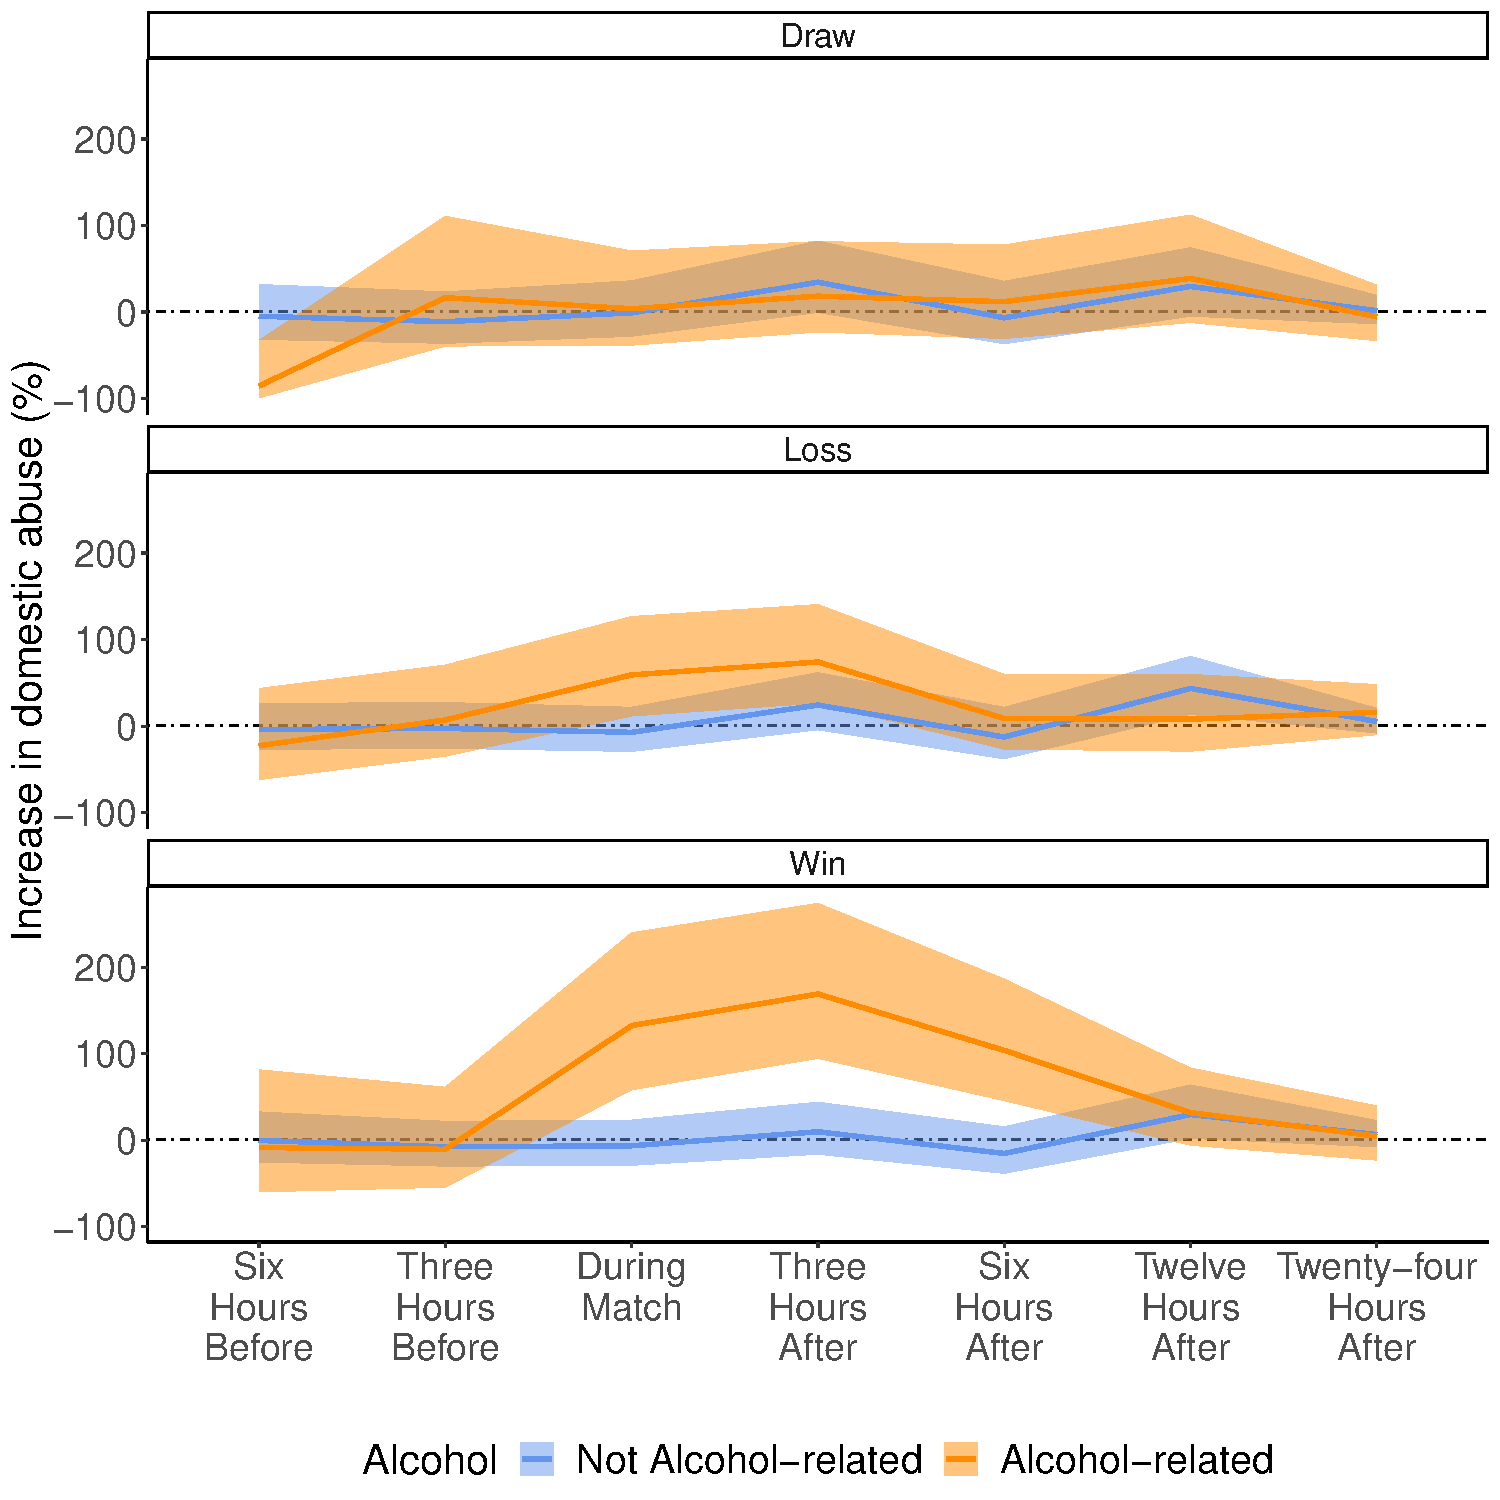
\includegraphics[width=0.75\textwidth]{Threehours.pdf}
\label{fig:threehours}
		\floatfoot{Note: Estimates are from two separate negative binomial regressions (based on tests of overdispersion) with year, month, day of week, three-hour period of day, Christmas, New Year's eve controls. Shaded area is 95\% CIs.}
\end{figure}


Our previous results revealed important differences in the effect of football on alcohol and non-alcohol cases, therefore we run two separate regressions for alcohol and non-alcohol related domestic abuse cases to analyse the temporal pattern of the increase. Figure \ref{fig:threehours} shows a plot of the estimated percentage increase from these negative binomial regressions, revealing a stark increase in alcohol-related domestic abuse on days of an England victory, starting in the three hour period of the match, peaking in the three-hour period afterwards, and gradually declining to its original level in the twenty-four hours following the victory. Interestingly, we also see a slight increase in non-alcohol related incidents twelve hours after a loss or a victory, probably reflecting the small increase in non-alcohol related domestic abuse after an England match day seen in Table \ref{specifications}.



%\\[-1.8ex] & \multicolumn{4}{c}{Reported number of domestic abuse cases} & Property-related  & Public Order  & Hate & Other violent \\ 
% & \multicolumn{4}{c}{} & Offences & Offences & incidents & Offences \\ 
%\\[-1.8ex] & Male to Male & Male to Female & Female to Female & Female to Male &  &  &  & \\ 
%\\[-1.8ex] & (1) & (2) & (3) & (4) & (5) & (6) & (7) & (8)\\ 


\begin{sidewaystable}
\centering
 \caption{The effect of football by perpetrator-victim subgroups and offence types, and the effect of rugby.}
   \label{table2}
    \scalebox{0.8}{
 \begin{threeparttable}
\begin{tabular}{@{\extracolsep{5pt}}lccccccccc} 
\\[-1.8ex]\hline 
\hline \\[-1.8ex] 
 & \multicolumn{9}{c}{\textit{Dependent variable:}} \\ 
\cline{2-10} 
\\[-1.8ex] & \multicolumn{5}{c}{Reported number of domestic abuse cases}  & Property-related  & Public Order  & Hate & Other violent \\ 
 & \multicolumn{4}{c}{} & Six Nations & Offences & Offences & incidents & Offences \\ 
\\[-1.8ex] & Male to Male & Male to Female & Female to Female & Female to Male & (Rugby) & &  &  & \\ 
\\[-1.8ex] & (1) & (2) & (3) & (4) & (5) & (6) & (7) & (8) & (9)\\ 
\hline \\[-1.8ex] 
 Alcohol & $-$0.825$^{***}$ & $-$0.870$^{***}$ & $-$0.858$^{***}$ & $-$0.808$^{***}$ & $-$0.862$^{***}$ & $-$0.981$^{***}$ & $-$0.922$^{***}$ & $-$0.934$^{***}$ & $-$0.902$^{***}$ \\ 
  & (0.101) & (0.034) & (0.080) & (0.080) & (0.031) & (0.065) & (0.080) & (0.115) & (0.040) \\ 
  Tournament on & 0.005 & 0.038$^{*}$ & $-$0.048 & 0.053 & 0.005 & 0.042 & 0.096$^{**}$ & 0.138$^{***}$ & 0.034 \\ 
  & (0.054) & (0.021) & (0.045) & (0.045) & (0.019) & (0.026) & (0.036) & (0.047) & (0.027) \\ 
  England win & $-$0.068 & $-$0.022 & $-$0.147 & 0.019 & 0.0001 & 0.052 & 0.234$^{**}$ & 0.073 & 0.094 \\ 
  & (0.165) & (0.066) & (0.135) & (0.135) & (0.035) & (0.074) & (0.095) & (0.136) & (0.077) \\ 
  England draw & 0.080 & 0.038 & 0.107 & 0.043 &  & 0.100 & $-$0.065 & $-$0.066 & 0.035 \\ 
  & (0.194) & (0.076) & (0.169) & (0.169) &  & (0.085) & (0.128) & (0.168) & (0.092) \\ 
  England lost & $-$0.063 & 0.065 & 0.117 & $-$0.036 & 0.056 & $-$0.042 & 0.075 & 0.011 & 0.089 \\ 
  & (0.162) & (0.064) & (0.136) & (0.136) & (0.055) & (0.078) & (0.100) & (0.139) & (0.078) \\ 
  After England & $-$0.036 & 0.093$^{**}$ & 0.025 & 0.152$^{*}$ & $-$0.010 & 0.052 & 0.161$^{**}$ & 0.141 & 0.108$^{**}$ \\ 
  & (0.103) & (0.040) & (0.082) & (0.082) & (0.031) & (0.047) & (0.062) & (0.084) & (0.048) \\ 
  Alcohol:Tournament on & $-$0.181$^{*}$ & $-$0.077$^{**}$ & $-$0.215$^{*}$ & $-$0.018 & $-$0.047 & 0.135 & $-$0.197$^{**}$ & $-$0.215$^{*}$ & $-$0.009 \\ 
  & (0.106) & (0.038) & (0.084) & (0.084) & (0.035) & (0.080) & (0.101) & (0.141) & (0.051) \\ 
  Alcohol:England win & 0.334 & 0.674$^{***}$ & 0.472 & 0.360 & 0.045 & 0.259 & 0.020 & 0.310 & 0.507$^{***}$ \\ 
  & (0.285) & (0.108) & (0.231) & (0.231) & (0.059) & (0.219) & (0.256) & (0.359) & (0.132) \\ 
  Alcohol:England draw & $-$0.282 & 0.031 & $-$0.580 & 0.071 &  & 0.060 & 0.374 & 0.393 & 0.360$^{*}$ \\ 
  & (0.411) & (0.138) & (0.313) & (0.313) &  & (0.264) & (0.303) & (0.431) & (0.161) \\ 
  Alcohol:England lost & 0.286 & 0.028 & $-$0.088 & 0.328 & $-$0.073 & 0.144 & 0.456$^{*}$ & $-$0.032 & 0.018 \\ 
  & (0.279) & (0.111) & (0.231) & (0.231) & (0.091) & (0.226) & (0.228) & (0.393) & (0.138) \\ 
  Alcohol:After England & 0.209 & 0.052 & $-$0.040 & $-$0.111 & $-$0.021 & 0.094 & 0.127 & 0.446$^{*}$ & 0.053 \\ 
  & (0.185) & (0.071) & (0.159) & (0.159) & (0.055) & (0.144) & (0.158) & (0.211) & (0.088) \\ 
 \hline \\[-1.8ex] 
Number of days & 3,017 & 3,017 & 3,017 & 3,017 & 3,017 & 3,017 & 3,017 & 3,017 & 3,017 \\ 
%Log Likelihood & $-$10,637.300 & $-$19,923.970 & $-$9,234.791 & $-$12,372.460 & $-$109,868.400 & $-$16,843.670 & $-$13,757.560 & $-$11,391.050 & $-$20,108.820 \\ 
%$\theta$ & 141.533  (111.012) & 59.918$^{***}$  (2.924) & 64.457$^{**}$  (31.740) & 60.289$^{***}$  (14.059) & 0.665$^{***}$  (0.005) & 40.698$^{***}$  (1.891) & 33.673$^{***}$  (2.784) & 24.170$^{***}$  (2.563) & 30.562$^{***}$  (1.167) \\ 
%Akaike Inf. Crit. & 21,406.600 & 39,979.950 & 18,601.580 & 24,876.910 & 219,864.900 & 33,819.350 & 27,647.120 & 22,914.090 & 40,349.640 \\ 
\hline 
\hline \\[-1.8ex] 
\textit{Note:}  & \multicolumn{9}{r}{$^{*}$p$<$0.1; $^{**}$p$<$0.05; $^{***}$p$<$0.01} \\ 
\end{tabular} 
\begin{tablenotes}
      \item[a] \textit{$^{*}$p$<$0.1; $^{**}$p$<$0.05; $^{***}$p$<$0.01}
      \item[b] \textit{Estimates are exponentiated coefficients from a series of negative binomial regressions (based on tests of overdispersion) with month, day of week, Christmas, New Year's eve controls interacted with alcohol; there was only one England rugby match that resulted in a draw between 2010 and 2018, therefore we excluded it from the data; standard errors in parentheses}
    \end{tablenotes}
\end{threeparttable} }
\end{sidewaystable}


Given the evidence for the gendered nature of domestic abuse, we find it instructive to test whether the effect varies by perpetrator-victim gender subgroup. The first four columns of Table \ref{table2} show the results from four negative binomial regressions, one for each offender-victim gender groups. These reveal a pronounced increase in the subgroup of Male to Female abuse (which comprises about 80\% of all domestic abuse cases in our data), where the number of reported alcohol-related cases increase by 67\%, 95\% CI [35\%--107\%] on England win days. While we see similar tendencies for alcohol-related cases in other gender subgroups on England win days, these coefficients are about half the size of the male to female effect, and are not statistically different from zero. 

Does this effect generalise to other sporting events, or is it specific to football?
It has been previously suggested that other popular sports, such as rugby have similar links with domestic abuse \cite{Brooks-Hay2018}. Rugby is the second most popular sport in England after football \cite{Ipsos2003}. Focusing on the Six Nations, a high-profile rugby tournament that takes place every year with the participation of England, Wales, Scotland, Ireland, France and Italy, we explored whether the reported number of domestic abuse cases increase on days when the England national rugby team plays. The results show no comparable effects for rugby matches (see column 5 in Table \ref{table2}), potentially stemming from differences in timing, media coverage, audience numbers, and the involvement of alcohol between the two tournaments. 


Our unique dataset further allows us to explore whether England games have similar effects on other types of criminal behaviours, apart from domestic abuse. Specifically, we are interested in how an England match day affects the number of reported property-related crimes (including burglary, theft and robbery), public order offences (behaviours that cause offence to the general public), hate crimes (hate incidents and any other racially or religiously aggravated crime), and other violent crimes (excluding cases of domestic abuse). Of particular interest is the effect of football on non-domestic violent crimes, since it is possible that alcohol-fuelled violence that follows an England victory is not limited to family and intimate partner relationships. The last four columns in Table \ref{table2} shows the results from a series of negative binomial regressions for different types of criminal behaviours. These reveal that while there is no evidence that England matches affect the number of reported property-related offences, we see an increase in the number of non-alcohol related public order offence cases on tournament days, when England wins, and on days after an England game. Hate incidents with no alcohol involvement also increase when the tournament is on. But most importantly, the effect of an England match on alcohol-related cases extends to other, non-domestic violent offences, resulting in a 55\%, 95\% [43\%--72\%] increase on days when England wins, and a smaller increase on days following an England match, the exact same pattern we have seen for domestic abuse. Further analysis reveals that the increase in these alcohol-related non-domestic violent crimes also predominantly comes from male to female cases (although male to male and female to male cases also contribute, see Table \ref{otherviolence_gender} in the Supplemental Material). While it is possible that a number of misclassified domestic abuse cases are reflected in this result (e.g, if the victim chooses not to disclose any relationship to the offender), but even if this was the case, taken together, these findings suggest that football and alcohol primarily make men more violent, and direct this violence overwhelmingly towards women.

A previous study by \cite{Kirby2014} have found that an England loss results in the most pronounced increase in domestic abuse (38\%), and a win or draw have a slightly smaller effect (26\%). They used daily counts of IPV in Lancashire from the months of the 2002, 2006, 2010 World Cups. Upon re-analysing their data by treating wins and draws as two separate variables (resulting in an improved model fit, see Table \ref{kirbyrep1}), we see a roughly similar effect for wins (45\%, 95\% CI [28\%--64\%]) and losses (39\%, 95\% CI [18\%--64\%]), and no effect when England draws. Our reanalysis replicates the win effect seen in the West Midlands data, though the absence of a loss effect remains a stark difference between the two studies.

\begin{table*}[!htb]
\centering
 \caption{Replication of Kirby et al. (2014) with an alternative specification}
   \label{kirbyrep1}
   \scalebox{0.85}{
 \begin{threeparttable}
\begin{tabular}{@{\extracolsep{5pt}}lcc} 
\\[-1.8ex]\hline 
\hline \\[-1.8ex] 
 & \multicolumn{2}{c}{\textit{Dependent variable:}} \\ 
\cline{2-3} 
\\[-1.8ex] & \multicolumn{2}{c}{Number of reported IPV cases per day} \\ 
\\ 
 & Original Model & Win/Draw Separate \\ 
\\[-1.8ex] & (1) & (2)\\ 
\hline \\[-1.8ex] 
 England windraw & 0.256$^{***}$ &  \\ 
  & (0.055) &  \\ 
  England win &  & 0.452$^{***}$ \\ 
  &  & (0.064) \\ 
  England draw &  & 0.032 \\ 
  &  & (0.073) \\ 
  England loss & 0.382$^{***}$ & 0.388$^{***}$ \\ 
  & (0.094) & (0.085) \\ 
  After England & 0.111$^{**}$ & 0.113$^{**}$ \\ 
  & (0.051) & (0.047) \\ 
 \hline \\[-1.8ex] 
Number of days & 92 & 92 \\ 
AIC & 714.980 & 704.356 \\ 
%BIC & 747.763 & 739.662 \\ 
%\hline 
\hline \\[-1.8ex] 
%\textit{Note:}  & \multicolumn{2}{r}{$^{*}$p$<$0.1; $^{**}$p$<$0.05; $^{***}$p$<$0.01} \\ 
\end{tabular} 
\begin{tablenotes}
      \item[a] \textit{$^{*}$p$<$0.1; $^{**}$p$<$0.05; $^{***}$p$<$0.01}
      \item[b] \textit{Estimates are exponentiated coefficients from a series of negative binomial regressions (based on tests of overdispersion) with year and day of week controls; standard errors in parentheses; data is only available during the tournament period}
    \end{tablenotes}
\end{threeparttable} }
\end{table*}


To explore the underlying reason for this discrepancy and test the robustness of our results, we find it instructive to break our analysis into specific tournament years for the two datasets (see Table \ref{kirbyrep2}). An interesting common pattern in both datasets is the large effect of England's victory over Slovenia in the group stage of the 2010 World Cup, which, after much anticipation, secured their progression to the next stage of the tournament. Equally, the subsequent loss against Germany in the knockout stage resulted in a substantial increase in the number of reported domestic abuse incidents, which is the only tournament year in our dataset where a loss effect appears. This is in line with findings from an earlier examination by \cite{Brimicombe2012}. As a further robustness check, we examine the sensitivity of the result to the exclusion of specific tournament years  (see Table \ref{robustness}), which shows that while the size of the England win effect varies, it is robust to the exclusion of specific years, and is not driven by an unusually large effect in one of the tournament years.

%\newpage

\begin{sidewaystable}[htp]
\centering
 \caption{Year subgroup regressions, Lancashire and West Midlands data}
   \label{kirbyrep2}
    \scalebox{0.8}{
 \begin{threeparttable}
\begin{tabular}{@{\extracolsep{5pt}}lcccccccc} 
\\[-1.8ex]\hline 
\hline \\[-1.8ex] 
 & \multicolumn{8}{c}{\textit{Dependent variable:}} \\ 
\cline{2-9} 
\\[-1.8ex] & \multicolumn{3}{c}{Number of IPV cases per day in Lancashire} & \multicolumn{5}{c}{Number of domestic abuse cases per day in West Midlands} \\ 
\\[-1.8ex] & \textit{negative} & \multicolumn{2}{c}{\textit{Poisson}} & \multicolumn{5}{c}{\textit{negative}} \\ 
 & \textit{binomial} & \multicolumn{2}{c}{\textit{}} & \multicolumn{5}{c}{\textit{binomial}} \\ 
 & 2002 & 2006 & 2010 & 2010 & 2012 & 2014 & 2016 & 2018 \\ 
\\[-1.8ex] & (1) & (2) & (3) & (4) & (5) & (6) & (7) & (8)\\ 
\hline \\[-1.8ex] 
 Tournament on &  &  &  & 0.074$^{*}$ & $-$0.066 & $-$0.048 & 0.035 & 0.089$^{*}$ \\ 
  &  &  &  & (0.041) & (0.085) & (0.044) & (0.041) & (0.044) \\ 
  England win & 0.596$^{***}$ & 0.297$^{***}$ & 0.916$^{***}$ & 0.050 & $-$0.237 &  & $-$0.008 & 0.061 \\ 
  & (0.152) & (0.077) & (0.114) & (0.155) & (0.175) &  & (0.151) & (0.077) \\ 
  England draw & 0.100 & 0.098 & $-$0.137 & $-$0.029 & 0.324 & $-$0.077 & $-$0.021 &  \\ 
  & (0.150) & (0.156) & (0.095) & (0.112) & (0.204) & (0.173) & (0.108) &  \\ 
  England loss & 0.200 & 0.373$^{***}$ & 0.568$^{***}$ & 0.174 & $-$0.127 & $-$0.042 & $-$0.155 & 0.066 \\ 
  & (0.232) & (0.117) & (0.106) & (0.140) & (0.212) & (0.124) & (0.154) & (0.088) \\ 
  After England & 0.253$^{**}$ & 0.122$^{*}$ & 0.024 & 0.070 & $-$0.008 & 0.007 & 0.038 & 0.140$^{**}$ \\ 
  & (0.101) & (0.070) & (0.065) & (0.082) & (0.125) & (0.103) & (0.081) & (0.060) \\ 
%  AlcoholYes &  &  &  & $-$0.853$^{***}$ & $-$0.803$^{***}$ & $-$0.704$^{***}$ & $-$0.725$^{***}$ & $-$0.743$^{***}$ \\ 
%  &  &  &  & (0.083) & (0.097) & (0.067) & (0.059) & (0.062) \\ 
  Tournament on:Alcohol &  &  &  & $-$0.093 & 0.076 & 0.063 & $-$0.163$^{**}$ & $-$0.068 \\ 
  &  &  &  & (0.101) & (0.162) & (0.076) & (0.072) & (0.078) \\ 
  England win:Alcohol &  &  &  & 2.558$^{***}$ & 0.756$^{*}$ &  & 0.348 & 0.460$^{***}$ \\ 
  &  &  &  & (0.277) & (0.314) &  & (0.257) & (0.123) \\ 
  England draw:Alcohol &  &  &  & 0.078 & $-$0.581 & 0.089 & 0.129 &  \\ 
  &  &  &  & (0.246) & (0.571) & (0.307) & (0.180) &  \\ 
  England loss:Alcohol &  &  &  & 0.748$^{**}$ & 0.301 & 0.048 & $-$0.289 & 0.160 \\ 
  &  &  &  & (0.259) & (0.372) & (0.206) & (0.322) & (0.149) \\ 
  After England:Alcohol &  &  &  & 0.128 & $-$0.072 & 0.068 & $-$0.112 & 0.188$^{*}$ \\ 
  &  &  &  & (0.183) & (0.254) & (0.171) & (0.144) & (0.102) \\ 
 \hline \\[-1.8ex] 
Number of days & 30 & 32 & 30 & 730 & 732 & 730 & 732 & 618 \\ 
%Log Likelihood & $-$112.494 & $-$101.847 & $-$107.268 & $-$2,315.879 & $-$2,259.612 & $-$2,604.474 & $-$2,614.295 & $-$2,237.868 \\ 
%$\theta$ & 57.581$^{*}$  (31.978) &  &  & 136.319$^{***}$  (31.759) & 55.994$^{***}$  (9.013) & 68.164$^{***}$  (8.225) & 109.262$^{***}$  (16.375) & 90.905$^{***}$  (12.959) \\ 
%Akaike Inf. Crit. & 246.989 & 225.694 & 236.536 & 4,731.757 & 4,619.224 & 5,304.947 & 5,328.590 & 4,563.737 \\ 
\hline 
\hline \\[-1.8ex] 
%\textit{Note:}  & \multicolumn{8}{r}{$^{*}$p$<$0.1; $^{**}$p$<$0.05; $^{***}$p$<$0.01} \\ 
\end{tabular} 
\begin{tablenotes}
      \item[a] \textit{$^{*}$p$<$0.1; $^{**}$p$<$0.05; $^{***}$p$<$0.01}
      \item[b] \textit{Estimates are exponentiated coefficients from a series of negative binomial or poisson regressions (based on tests of overdispersion). The first three regressions have day of week control, the rest of the regressions have month, day of week, Christmas, New Year's eve controls interacted with alcohol; standard errors in parentheses}
    \end{tablenotes}
\end{threeparttable} }
\end{sidewaystable}

\newpage



\begin{table}[htp]
\centering
 \caption{Robustness of the result: sensitivity to the exclusion of specific years}
  \label{robustness}
 \scalebox{0.8}{
  \begin{threeparttable}
\begin{tabular}{@{\extracolsep{5pt}}lccccc} 
\\[-1.8ex]\hline 
\hline \\[-1.8ex] 
 & \multicolumn{5}{c}{\textit{Dependent variable:}} \\ 
 \cline{2-6} 
\\[-1.8ex] 
  & \multicolumn{5}{c}{Number of domestic abuse cases per day} \\ 
 \\
%\\[-1.8ex] & \multicolumn{5}{c}{N} \\ 
 & 2018 & 2016 & 2014 & 2012 & 2010 \\ 
  &  excluded & excluded & excluded & excluded & excluded \\ 
\\[-1.8ex] & (1) & (2) & (3) & (4) & (5)\\ 
\hline \\[-1.8ex] 
%Alcohol & $-$0.862$^{***}$ & $-$0.862$^{***}$ & $-$0.862$^{***}$ & $-$0.863$^{***}$ & $-$0.867$^{***}$ \\ 
  & (0.033) & (0.033) & (0.032) & (0.031) & (0.033) \\ 
  Tournament on & 0.018 & 0.015 & 0.027 & 0.030 & $-$0.003 \\ 
  & (0.022) & (0.025) & (0.025) & (0.022) & (0.025) \\ 
  England win & $-$0.093 & $-$0.047 & $-$0.029 & 0.019 & $-$0.051 \\ 
  & (0.097) & (0.068) & (0.062) & (0.066) & (0.067) \\ 
  England draw & 0.038 & 0.077 & 0.057 & 0.004 & 0.046 \\ 
  & (0.072) & (0.091) & (0.078) & (0.075) & (0.088) \\ 
  England loss & 0.030 & 0.066 & 0.053 & 0.054 & 0.013 \\ 
  & (0.079) & (0.065) & (0.069) & (0.062) & (0.065) \\ 
  After England & 0.057 & 0.080$^{*}$ & 0.088$^{**}$ & 0.099$^{**}$ & 0.071$^{*}$ \\ 
  & (0.048) & (0.042) & (0.040) & (0.039) & (0.042) \\ 
  Alcohol:Tournament on & $-$0.086$^{**}$ & $-$0.037 & $-$0.118$^{***}$ & $-$0.092$^{**}$ & $-$0.048 \\ 
  & (0.039) & (0.046) & (0.047) & (0.040) & (0.042) \\ 
  Alcohol:England win & 0.884$^{***}$ & 0.674$^{***}$ & 0.609$^{***}$ & 0.574$^{***}$ & 0.511$^{***}$ \\ 
  & (0.163) & (0.109) & (0.100) & (0.105) & (0.107) \\ 
  Alcohol:England draw & $-$0.046 & $-$0.141 & $-$0.048 & 0.055 & $-$0.017 \\ 
  & (0.130) & (0.179) & (0.141) & (0.131) & (0.151) \\ 
  Alcohol:England loss & 0.014 & 0.139 & 0.131 & 0.078 & 0.039 \\ 
  & (0.134) & (0.107) & (0.116) & (0.103) & (0.109) \\ 
  Alcohol:After England & $-$0.065 & 0.096 & 0.050 & 0.054 & 0.050 \\ 
  & (0.086) & (0.073) & (0.071) & (0.067) & (0.071) \\ 
 \hline \\[-1.8ex] 
Number of days & 2,708 & 2,651 & 2,652 & 2,651 & 2,652 \\ 
%Log Likelihood & $-$18,626.890 & $-$18,243.850 & $-$18,269.330 & $-$18,506.890 & $-$18,533.610 \\ 
%$\theta$ & 60.431$^{***}$  (2.862) & 58.624$^{***}$  (2.761) & 62.319$^{***}$  (3.016) & 67.975$^{***}$  (3.245) & 59.902$^{***}$  (2.752) \\ 
%Akaike Inf. Crit. & 37,381.780 & 36,615.700 & 36,666.660 & 37,141.780 & 37,195.210 \\ 
\hline 
%\hline \\[-1.8ex] 
%\textit{Note:}  & \multicolumn{6}{r}{$^{*}$p$<$0.1; $^{**}$p$<$0.05; $^{***}$p$<$0.01} \\ 
%\end{tabular} 
%\end{table} 

\end{tabular}
\begin{tablenotes}
      \item[a] \textit{$^{*}$p$<$0.1; $^{**}$p$<$0.05; $^{***}$p$<$0.01}
      \item[b] \textit{Estimates are exponentiated coefficients from a series of negative binomial regressions (based on tests of overdispersion)  with year, month, day of week, Christmas, New Year's eve controls interacted by alcohol; standard errors in parentheses}
    \end{tablenotes}
\end{threeparttable} } 
\end{table}




%\textbf{\textit{Characteristics of domestic abuse perpetrated on England days.}} Our data further allows us to explore the characteristics of alcohol-related domestic abuse perpetrated on England match days. First, using a series of logistic regressions, we investigate whether these cases are more likely to be newly reported (with no earlier record for the same victim-offender pair in our dataset), happen in a residential dwelling as opposed to a public location, or result in an injury. We find no evidence that domestic abuse cases perpetrated on England match days are more likely to be newly reported (see Table \ref{Characteristics1} in the Supplemental Material), compared to domestic abuse cases occurring on non-match days. Interestingly, our results indicate that, compared to non-match days, reported cases are more likely to be perpetrated in public on England loss days, but not on England win days, and that this effect does not differ by alcohol-involvement in the case. Non-alcohol related cases reported on England loss days are also more likely to result in an injury, a pattern that is absent from alcohol-related cases.

%Next, we turn to repeated cases of domestic abuse (multiple cases with the same victim-offender pair). Domestic abuse is rarely a one-off incident, and reported repeat cases allow us to explore the characteristics of domestic abuse that occurs on match days in more detail. We are interested in whether the number of days elapsed between two consecutive cases is affected by England football matches. For example, it is possible that England match days bring reported cases of domestic abuse forward, which would have otherwise happened at a later point in time. We investigate this question with two negative binomial regressions, where the outcome variables are the number of days elapsed since the last reported case, and the number of days until the next case, respectively. In addition, using all reported cases, we explore whether the number of hours elapsed before reporting the case is affected by England match days.


%The results shown in Table \ref{Characteristics2} in the Supplemental Material show that non-alcohol related cases perpetrated on England loss days occur fewer days after the previous incident compared to non-alcohol repeat cases reoccurring on non-match days. Non-alcohol related domestic abuse cases perpetrated on England win days are more likely to be followed by another case of abuse in fewer days compared to cases occurring on non-match days, and this pattern is absent from alcohol-related cases. Interestingly, non-alcohol related cases perpetrated on England loss days are likely to be reported after fewer hours, compared to non-alcohol related abuse perpetrated on non-match days. 


%Finally, using the sample of repeated cases, we explore whether previously non-alcohol related cases are more likely to reoccur as alcohol-related abuse on England match days. We investigate this question using a logistic regression, controlling for the type of the previous case (alcohol/non-alcohol related). The results shown in Table \ref{alctrans} in the Supplemental Material that on England win days, there is an increased likelihood of an alcohol-related case occurring, irrespective of whether the previous case was alcohol-related or not. Taken together, these results indicate that apart from the higher likelihood of alcohol-involvement, domestic abuse that follows an England victory is not characteristically different from domestic abuse perpetrated on other days during the year.

\clearpage

\section*{Discussion}

We have shown that an England victory in a national football tournament is followed by a 61\% increase in the reported number of alcohol-related domestic abuse cases, and that the temporal pattern of the increase suggests a causal mechanism. The effect is entirely limited to alcohol-related abuse, even though alcohol-related domestic abuse cases comprise only 23\% of all domestic abuse in our dataset. As such, we see this as strong quantitative evidence that alcohol plays an instrumental role in the relationship between football and domestic abuse. This effect is exclusively limited to male-perpetrated domestic abuse, implicating a victory-induced violent expression of masculinity coupled with alcohol consumption as the pathway by which football increases abuse. In line with this, anecdotal evidence suggests that alcohol consumption increases following an England victory \cite{Davies2018}. 


It had been previously suggested that the apparent link between football and domestic abuse can be explained by other factors, including high-profile events taking place around the time of the match, increased policing on England match days, and the effect of awareness campaigns before the tournaments \cite{Brooks-Hay2018}. However, our three-hour analysis strongly suggests that the effect is causal, further supported by the fact that the majority of England match days were allocated randomly. In addition, we could expect that higher levels of policing on England match days would result in an increased number of recorded cases perpetrated outside, and that a successful pre-tournament awareness campaign would result in an increase in the number of newly reported cases. Our results presented in Table \ref{Characteristics1} in the Supplemental Material do not support either of these alternative hypotheses in that we do not see more newly reported, or publicly perpetrated cases of abuse on England win days. Furthermore, it is unclear why the effect of other events, different policing practices, or awareness campaigns would depend on the result of the match. 

One limitation of our analysis is that it only relies on cases recorded by the police, while the vast majority of domestic abuse cases do not get reported. Future investigations of the link between football, alcohol, and domestic abuse should aim to combine data from various sources (e.g., police data, calls to shelters, hospital admissions, etc.) to address the potential bias arising from underreporting. 



% Replicating the results of a previous US study, we found that it is male to female abuse that is affected by a sporting event \cite{Card2011}. In the same study, the effect of the match did not depend on alcohol-involvement in the abuse case, and the increase was driven by unexpected losses. In contrast, we find that in the context of England and football, it is a victory that results in the largest increase, and that alcohol involvement is critical. This discrepancy most likely stems from the contextual differences between the two studies (England, football, national tournaments vs. US, American football, NFL matches). 


 Our study represent the most extensive quantitative investigation of the link between football and domestic abuse up to date. We have shown that our findings are largely in line with results from previous, smaller-scale investigations from England (the main difference being the lack of an England loss effect in our sample), and substantially extend them in highlighting the instrumental role alcohol plays in the relationship between football and domestic abuse. While the effect of a victory or loss is likely to be highly specific to the context of a particular match (e.g., group stage or knockout stage, previous performance of the team, weather on the day, etc.), the estimated effect of an England victory on the number of reported domestic abuse cases is robust to different model specifications, using data from a different geographical area, and the exclusion of specific tournament years. 


Based on the pre-match betting odds, all of the England victories were expected in our dataset. This suggests that in the context of England's participation in national football tournaments, it is living up to the expectations of the fans that results in largest emotional effect and affects levels of alcohol consumption. Indeed, English newspapers' narratives about the team's performance in these tournaments are characterised with high levels of optimism, expectation and yearning for the glory of the 1966 World Cup \cite{Vincent2010}. Previous research has demonstrated how the vicarious experience of watching their team play can increase supporter's testosterone and cortisol levels, even when they expect their team to win, suggested to be an adaptive response to the perceived threat to one's social identity \cite{VanderMeij2012}. 






%It is perhaps surprising that while we found no evidence for an increase in the reported number of domestic abuse cases on England loss days (see Table \ref{specifications}), domestic abuse perpetrated on these days seems to be characteristically different from domestic abuse perpetrated on other days in terms of location, resulting injury, and time delay before reporting. While these findings should be interpreted with caution due to the pervasive problem of underreporting, the results suggest differences in the effect of England wins and losses on domestic abuse.


For victims, domestic abuse does not occur once every four years following a football match, but is a lived experience of constant fear \cite{Brooks-Hay2018}. Nevertheless, our results provide a deeper understanding of the contexts that can be conducive to abuse. In particular, these findings illuminate that the experience of ``national success'' in a highly male-dominated sport is a breeding ground for male-perpetrated, alcohol-related domestic abuse.

\newpage




%\section*{Data availability statement}
%
%The data that support the findings of this study are available from West Midlands Police
%but restrictions apply to the availability of these data, which were used under license
%for the current study by researchers with security vetting from the police, and so are not publicly available. Data are however available from the authors upon reasonable request and with permission of West Midlands Police.
%
%\section*{Code availability}
%
%The code for producing the results can be accessed \href{https://osf.io/kg9yr/?view_only=172a33b467bd4566b2e5dea0e2f59f8c}{here}. 

\clearpage
\bibliography{football_refs}
\newpage

%\theendnotes

\clearpage



\section*{Supplemental Material}

\renewcommand{\thetable}{S\arabic{table}}
\renewcommand{\thefigure}{S\arabic{figure}}
\setcounter{table}{0}
\setcounter{figure}{0}

\begin{table}[htp]
\centering
 \caption{Non-domestic violent cases by gender}
  \label{otherviolence_gender}
 \scalebox{0.9}{
   \begin{threeparttable}
\begin{tabular}{@{\extracolsep{5pt}}lcccc} 
\\[-1.8ex]\hline 
\hline \\[-1.8ex] 
 & \multicolumn{4}{c}{\textit{Dependent variable:}} \\ 
\cline{2-5} 
\\[-1.8ex] & \multicolumn{4}{c}{Number of other violent abuse cases per day} \\ 
\\
 & Male & Male & Female & Female \\ 
 & to Male & to Female & to Female & to Male \\ 
\\[-1.8ex] & (1) & (2) & (3) & (4)\\ 
\hline \\[-1.8ex] 
% Alcohol & $-$0.900$^{***}$ & $-$0.891$^{***}$ & $-$0.864$^{***}$ & $-$0.921$^{***}$ \\ 
%  & (0.048) & (0.033) & (0.080) & (0.066) \\ 
  Tournament on & 0.037 & 0.050$^{**}$ & 0.041 & 0.051 \\ 
  & (0.026) & (0.021) & (0.038) & (0.036) \\ 
  England win & 0.013 & 0.019 & $-$0.031 & 0.174 \\ 
  & (0.082) & (0.067) & (0.111) & (0.112) \\ 
  England draw & 0.089 & 0.012 & 0.115 & 0.042 \\ 
  & (0.094) & (0.078) & (0.139) & (0.132) \\ 
  England loss & 0.018 & 0.028 & 0.088 & 0.118 \\ 
  & (0.082) & (0.066) & (0.114) & (0.108) \\ 
  After England & 0.085 & 0.070 & 0.181$^{**}$ & 0.149$^{**}$ \\ 
  & (0.050) & (0.042) & (0.071) & (0.067) \\ 
  Alcohol:Tournament on & $-$0.027 & $-$0.086$^{**}$ & $-$0.077 & $-$0.167$^{**}$ \\ 
  & (0.055) & (0.038) & (0.087) & (0.073) \\ 
  Alcohol:England win & 0.391$^{**}$ & 0.613$^{***}$ & 0.441$^{*}$ & $-$0.114 \\ 
  & (0.158) & (0.109) & (0.251) & (0.199) \\ 
  Alcohol:England draw & 0.071 & 0.102 & 0.127 & $-$0.337 \\ 
  & (0.192) & (0.137) & (0.361) & (0.254) \\ 
  Alcohol:England loss & 0.296$^{*}$ & 0.057 & $-$0.023 & 0.027 \\ 
  & (0.153) & (0.112) & (0.237) & (0.207) \\ 
  Alcohol:After England & 0.208$^{*}$ & 0.053 & $-$0.119 & $-$0.158 \\ 
  & (0.100) & (0.072) & (0.163) & (0.136) \\ 
 \hline \\[-1.8ex] 
Number of days & 3,017 & 3,017 & 3,017 & 3,017 \\ 
%Log Likelihood & $-$17,204.240 & $-$21,360.820 & $-$13,708.300 & $-$14,378.320 \\ 
%$\theta$ & 44.231$^{***}$  (2.800) & 43.449$^{***}$  (1.546) & 24.998$^{***}$  (1.919) & 35.978$^{***}$  (3.376) \\ 
%Akaike Inf. Crit. & 34,540.480 & 42,853.640 & 27,548.590 & 28,888.630 \\ 
\hline 
\hline \\[-1.8ex] 
%\textit{Note:}  & \multicolumn{4}{r}{$^{*}$p$<$0.1; $^{**}$p$<$0.05; $^{***}$p$<$0.01} \\ 
\end{tabular} 
\begin{tablenotes}
     \item[a] \textit{$^{*}$p$<$0.1; $^{**}$p$<$0.05; $^{***}$p$<$0.01}
      \item[b] \textit{Estimates are exponentiated coefficients from a series of negative binomial regressions (based on tests of overdispersion)  with year, month, day of week, Christmas, New Year's eve controls interacted with alcohol; standard errors in parentheses}
    \end{tablenotes}
\end{threeparttable} }
\end{table}

\newpage



%\newpage
%
%\begin{table}[htp]
%\centering
% \scalebox{0.85}{
%  \begin{threeparttable}
% \caption{The effect of England matches in the Six Nations rugby tournament on domestic abuse}
%  \label{rugby}
%\begin{tabular}{@{\extracolsep{5pt}}lc} 
%\\[-1.8ex]\hline 
%\hline \\[-1.8ex] 
% & \multicolumn{1}{c}{\textit{Dependent variable:}} \\ 
%\cline{2-2} 
%\\[-1.8ex] & Number of reported \\ 
%& domestic abuse cases per day \\
%\hline \\[-1.8ex] 
%% Alcohol & $-$0.862$^{***}$ \\ 
%%  & (0.031) \\ 
%  Tournament on & 0.005 \\ 
%  & (0.019) \\ 
%  England win & 0.0001 \\ 
%  & (0.035) \\ 
%  England loss & 0.056 \\ 
%  & (0.055) \\ 
%  After England & $-$0.010 \\ 
%  & (0.031) \\ 
%  Alcohol:Tournament on & $-$0.047 \\ 
%  & (0.035) \\ 
%  Alcohol:England win & 0.045 \\ 
%  & (0.059) \\ 
%  Alcohol:England loss & $-$0.073 \\ 
%  & (0.091) \\ 
%  Alcohol:After England & $-$0.021 \\ 
%  & (0.055) \\ 
% \hline \\[-1.8ex] 
%Number of days & 3,017 \\ 
%%Log Likelihood & $-$20,935.710 \\ 
%%$\theta$ & 60.091$^{***}$  (2.639) \\ 
%%Akaike Inf. Crit. & 41,999.420 \\ 
%%\hline 
%\hline \\[-1.8ex] 
%%\textit{Note:}  & \multicolumn{1}{r}{$^{*}$p$<$0.1; $^{**}$p$<$0.05; $^{***}$p$<$0.01} \\ 
%\end{tabular} 
%\begin{tablenotes}
%      \item[a] \textit{$^{*}$p$<$0.1; $^{**}$p$<$0.05; $^{***}$p$<$0.01}
%      \item[b] \textit{Estimates are from a series of negative binomial regressions (based on tests of overdispersion)  with year, month, day of week, Christmas, New Year's eve controls interacted by alcohol; there was only one England rugby match that resulted in a draw between 2010 and 2018, therefore we excluded it from the data; standard errors in parentheses}
%    \end{tablenotes}
%\end{threeparttable} } 
%\end{table}
%
%
%\newpage
%
%\begin{table}[htp]
%\centering
% \caption{Non domestic abuse incidents that are about power}
%  \label{otherabuse}
%  \scalebox{0.9}{
%  \begin{threeparttable}
%\begin{tabular}{@{\extracolsep{5pt}}lcc} 
%\\[-1.8ex]\hline 
%\hline \\[-1.8ex] 
% & \multicolumn{2}{c}{\textit{Dependent variable:}} \\ 
%\cline{2-3} 
%  \\[-1.8ex] & \multicolumn{2}{c}{Number of cases per day} \\ 
%\\
%& Sexual & Other \\ 
% & Offences & Abuse \\
%\\[-1.8ex] & (1) & (2)\\ 
%\hline \\[-1.8ex] 
%% Alcohol & $-$0.955$^{***}$ & $-$0.950$^{***}$ \\ 
%%  & (0.146) & (0.075) \\ 
%  Tournament on & 0.079 & 0.078$^{*}$ \\ 
%  & (0.068) & (0.042) \\ 
%  England win & $-$0.172 & $-$0.073 \\ 
%  & (0.217) & (0.132) \\ 
%  England draw & $-$0.062 & 0.175 \\ 
%  & (0.253) & (0.148) \\ 
%  England loss & $-$0.220 & 0.153 \\ 
%  & (0.223) & (0.132) \\ 
%  After England & $-$0.035 & 0.095 \\ 
%  & (0.134) & (0.081) \\ 
%  Alcohol:Tournament on & $-$0.121 & $-$0.069 \\ 
%  & (0.157) & (0.093) \\ 
%  Alcohol:England win & 0.191 & 0.166 \\ 
%  & (0.462) & (0.274) \\ 
%  Alcohol:England draw & 0.781 & $-$0.252 \\ 
%  & (0.503) & (0.346) \\ 
%  Alcohol:England loss & 0.011 & $-$0.111 \\ 
%  & (0.483) & (0.285) \\ 
%  Alcohol:After England & 0.114 & $-$0.172 \\ 
%  & (0.287) & (0.182) \\ 
% \hline \\[-1.8ex] 
%Number of days & 3,017 & 3,017  \\ 
%%Log Likelihood & $-$11,443.050 & $-$16,185.970 \\ 
%%$\theta$ & 4.549$^{***}$  (0.179) & 10.699$^{***}$  (0.400) \\ 
%%Akaike Inf. Crit. & 23,018.100 & 32,503.940 \\ 
%\hline 
%\hline \\[-1.8ex] 
%%\textit{Note:}  & \multicolumn{2}{r}{$^{*}$p$<$0.1; $^{**}$p$<$0.05; $^{***}$p$<$0.01} \\ 
%\end{tabular}
%\begin{tablenotes}
%      \item[a] \textit{$^{*}$p$<$0.1; $^{**}$p$<$0.05; $^{***}$p$<$0.01}
%      \item[b] \textit{Estimates are from a series of negative binomial regressions (based on tests of overdispersion)  with year, month, day of week, Christmas, New Year's eve controls interacted by alcohol; standard errors in parentheses}
%    \end{tablenotes}
%\end{threeparttable} } 
%\end{table}
%\newpage




\begin{table}[htp]
\centering
 \caption{Characteristics of domestic abuse cases reported on match days}
  \label{Characteristics1}
  \scalebox{0.9}{
  \begin{threeparttable}
\begin{tabular}{@{\extracolsep{5pt}}lccc} 
\\[-1.8ex]\hline 
\hline \\[-1.8ex] 
 & \multicolumn{3}{c}{\textit{Dependent variable:}} \\ 
\cline{2-4} 
\\[-1.8ex] & Newly & Public &  \\ 
& Reported & Location &  \\ 
& Yes=1, & Yes=1, &  \\ 
& No=0 & No=0 & \\ 
\\[-1.8ex] & (1) & (2) & \\ 
\hline \\[-1.8ex] 
% Alcohol=Yes & $-$0.030 & 0.001 & 0.427$^{***}$ \\ 
%  & (0.059) & (0.081) & (0.058) \\ 
  Tournament on & $-$0.037 & 0.021 & \\ 
  & (0.030) & (0.037) &  \\ 
  England win & 0.011 & 0.167 & \\ 
  & (0.089) & (0.110) &  \\ 
  England draw & 0.082 & 0.014 &  \\ 
  & (0.121) & (0.138) &  \\ 
  England loss & $-$0.099 & 0.337$^{***}$ &  \\ 
  & (0.086) & (0.099) &  \\ 
  After England & 0.035 & 0.070 & \\ 
  & (0.056) & (0.068) &  \\ 
  Alcohol:Tournament on & 0.087 & 0.063 &  \\ 
  & (0.060) & (0.080) &  \\ 
  Alcohol:England win & 0.093 & 0.104 &  \\ 
  & (0.156) & (0.196) &  \\ 
  Alcohol:England draw & $-$0.151 & $-$0.016 &  \\ 
  & (0.233) & (0.306) &  \\ 
  Alcohol:England loss & 0.221 & 0.044 & \\ 
  & (0.171) & (0.198) &  \\ 
  Alcohol:After England & $-$0.036 & 0.042 &  \\ 
  & (0.108) & (0.143) &  \\ 
 \hline \\[-1.8ex] 
Number of cases & 251,976 & 279,777 & \\ 
\hline \\[-1.8ex] 
%\textit{Note:}  & \multicolumn{3}{r}{$^{*}$p$<$0.1; $^{**}$p$<$0.05; $^{***}$p$<$0.01} \\ 
\end{tabular} 
\begin{tablenotes}
      \item[a] \textit{$^{*}$p$<$0.1; $^{**}$p$<$0.05; $^{***}$p$<$0.01}
      \item[b] \textit{Estimates are log odds from a series of logistic regressions with year, month, day of week, Christmas, New Year's eve controls interacted by alcohol, where every observation is a reported domestic abuse case; cases that happened in 2010 were excluded from the first regression; standard errors clustered by victim-offender pairs are in parentheses}
    \end{tablenotes}
\end{threeparttable} } 
\end{table}
\newpage

%\begin{table}[htp]
%\centering
%  \caption{Characteristics of domestic abuse cases reported on match days II}
%    \label{Characteristics2}
% \scalebox{0.9}{
%  \begin{threeparttable}
%\begin{tabular}{@{\extracolsep{5pt}}lccc} 
%\\[-1.8ex]\hline 
%\hline \\[-1.8ex] 
% & \multicolumn{3}{c}{\textit{Dependent variable:}} \\ 
%\cline{2-4} 
%\\[-1.8ex] & Days & Days & Hours \\ 
% & since last & until next & until reported \\
%\\[-1.8ex] & (1) & (2) & (3)\\ 
%\hline \\[-1.8ex] 
%% Alcohol & 0.103$^{*}$ & 0.057 & $-$0.839$^{***}$ \\ 
%%  & (0.054) & (0.050) & (0.189) \\ 
%  Tournament on & $-$0.014 & $-$0.047$^{*}$ & 0.080 \\ 
%  & (0.028) & (0.028) & (0.063) \\ 
%  England win & 0.016 & $-$0.340$^{***}$ & $-$0.098 \\ 
%  & (0.082) & (0.095) & (0.162) \\ 
%  England draw & $-$0.017 & $-$0.111 & 0.034 \\ 
%  & (0.096) & (0.105) & (0.208) \\ 
%  England loss & $-$0.163$^{*}$ & $-$0.104 & $-$0.560$^{***}$ \\ 
%  & (0.087) & (0.087) & (0.170) \\ 
%  After England & 0.052 & $-$0.139$^{**}$ & $-$0.243$^{**}$ \\ 
%  & (0.054) & (0.055) & (0.108) \\ 
%  Alcohol:Tournament on & 0.026 & 0.025 & 0.200 \\ 
%  & (0.057) & (0.056) & (0.197) \\ 
%  Alcohol:England win & $-$0.119 & 0.358$^{**}$ & 0.152 \\ 
%  & (0.146) & (0.159) & (0.450) \\ 
%  Alcohol:England draw & $-$0.266 & $-$0.116 & $-$0.935$^{**}$ \\ 
%  & (0.231) & (0.208) & (0.390) \\ 
%  Alcohol:England loss & 0.277$^{*}$ & 0.114 & 0.552 \\ 
%  & (0.159) & (0.166) & (0.654) \\ 
%  Alcohol:After England & $-$0.104 & 0.147 & $-$0.265 \\ 
%  & (0.106) & (0.102) & (0.297) \\ 
% \hline \\[-1.8ex] 
%Number of cases & 95,091 & 95,091 & 272,793 \\ 
%%\hline 
%\hline \\[-1.8ex] 
%%\textit{Note:}  & \multicolumn{3}{r}{$^{*}$p$<$0.1; $^{**}$p$<$0.05; $^{***}$p$<$0.01} \\ 
%\end{tabular}
%\begin{tablenotes}
%      \item[a] \textit{$^{*}$p$<$0.1; $^{**}$p$<$0.05; $^{***}$p$<$0.01}
%      \item[b] \textit{Estimates are exponentiated coefficients from a series of negative binomial regressions (based on tests of overdispersion)  with year, month, day of week, Christmas, New Year's eve controls interacted by alcohol, where every observation is a reported domestic abuse case; for each regression, we excluded the upper 2.5\% of the outcome variable; standard errors clustered by victim-offender pairs are in parentheses}
%    \end{tablenotes}
%\end{threeparttable} } 
%\end{table}
%
%\newpage
%
%
%\begin{table}[htp]
%\centering
%  \caption{Alcohol transition on England match days}
%    \label{alctrans}
% \scalebox{0.9}{
%  \begin{threeparttable}
%\begin{tabular}{@{\extracolsep{5pt}}lc} 
%\\[-1.8ex]\hline 
%\hline \\[-1.8ex] 
% & \multicolumn{1}{c}{\textit{Dependent variable:}} \\ 
%\cline{2-2} 
%	\\[-1.8ex] & Alcohol-involvement in case \\ 
%& Yes=1, \\ 
%& No=0 \\ 
%\hline \\[-1.8ex] 
% Tournament on & $-$0.134$^{**}$ \\ 
%  & (0.062) \\ 
%  England win & 0.443$^{***}$ \\ 
%  & (0.157) \\ 
%  England draw & 0.368$^{*}$ \\ 
%  & (0.201) \\ 
%  England loss & $-$0.113 \\ 
%  & (0.180) \\ 
%  After England & 0.041 \\ 
%  & (0.114) \\ 
%%  Previous\_alc=Yes & 1.670$^{***}$ \\ 
%%  & (0.120) \\ 
%  Tournament on:Previous alcohol & $-$0.051 \\ 
%  & (0.100) \\ 
%  England win:Previous alcohol & $-$0.110 \\ 
%  & (0.277) \\ 
%  England draw:Previous alcohol & $-$0.365 \\ 
%  & (0.372) \\ 
%  England lost:Previous alcohol & 0.179 \\ 
%  & (0.292) \\ 
%  After England:Previous alcohol & 0.066 \\ 
%  & (0.180) \\ 
% \hline \\[-1.8ex] 
%Number of cases & 97,292 \\ 
%%R$^{2}$ & 0.208 \\ 
%%$\chi^{2}$ & 14,868.240$^{***}$ (df = 65) \\ 
%%\hline 
%\hline \\[-1.8ex] 
%%\textit{Note:}  & \multicolumn{1}{r}{$^{*}$p$<$0.1; $^{**}$p$<$0.05; $^{***}$p$<$0.01} \\ 
%\end{tabular} 
%\begin{tablenotes}
%      \item[a] \textit{$^{*}$p$<$0.1; $^{**}$p$<$0.05; $^{***}$p$<$0.01}
%      \item[b] \textit{Estimates are log odds from a logistic regression with year, month, day of week, Christmas, New Year's eve controls interacted by alcohol involvement of the previous case, where every observation is a reported domestic abuse case; standard errors clustered by victim-offender pairs are in parentheses}
%    \end{tablenotes}
%\end{threeparttable} } 
%\end{table}



\end{document}

